%实验报告-重力加速度的测量

%文档类型
\documentclass[a4paper]{article}%A4纸,文档类型为论文

%宏包
%文字设置
\usepackage[UTF8]{ctex}%处理中文
\usepackage{xeCJK}%处理中文
\usepackage{fontspec,xunicode,xltxtra}%字体设置
%文档&排版设置
\usepackage{titlesec}%自定义章节标题样式
\usepackage{multicol}%分栏
\usepackage{hyperref}%超链接设置\daleth 
\usepackage{multirow,makecell}%制作复杂表格
\usepackage{booktabs}%画三线表要用
\usepackage{float}%图片、表格等位置浮动排版
\usepackage{indentfirst}%首行缩进
\usepackage{graphicx,subfigure}%图片插入
\usepackage{listings}%代码高亮
\usepackage{xcolor}
\usepackage{appendix}%附录
\usepackage{fancyhdr}%页眉页脚
\usepackage{geometry}%页边距
\usepackage{caption}
%数学
\usepackage{amsmath,amssymb}%公式
\usepackage{amsfonts,mathrsfs,txfonts}%数学字体
\usepackage{array}%矩阵
\usepackage{gensymb}%角度单位“度”的命令:\degree

\geometry{a4paper,scale=0.8}%设置了纸张为a4,并且版心占页面长度的比例为80%;scale也可以改为ratio,表示版面边距占页面长度的比例.
\hypersetup{colorlinks=true,linkcolor=black,citecolor=black}%去掉目录等超链接所带的红框,并让参考文献的引用颜色为黑色
\setlength{\parindent}{2em}%首行缩进2字符
\lstset{
    columns=fixed,
    numbers=left, % 在左侧显示行号
    numberstyle=\footnotesize\color{darkgray},% 设定行号格式
    backgroundcolor=\color[RGB]{245,245,244},% 设定背景颜色
    keywordstyle=\color[RGB]{40,40,255},% 设定关键字颜色
    numberstyle=\color[RGB]{0,192,192},%行号数字样式
    commentstyle=\it\color[RGB]{0,96,96},% 设置代码注释的格式
    stringstyle=\rmfamily\slshape\color[RGB]{128,0,0},% 设置字符串格式
}
\pagestyle{fancy}%页眉页脚
\fancyhead{}%清空页眉
\fancyhead[C]{\emph{实验报告I:重力加速度的测量}}


\newcommand{\kaiti}{\CJKfamily{STKaiti}} % 楷体:\kaiti或\emph
\newcommand{\fs}{\CJKfamily{STFangsong}} % 仿宋:\fs或\fangsong
%黑体:\heiti

\newcommand{\suo}{\indent}%缩进2个字符

\title{\heiti{实验报告}}%标题
\author{{\emph{李佩哲}}}
\date{\emph{\small\today}}

\begin{document}
\begin{center}
\center{\bf{\LARGE{实验报告}\\\large{重力加速度的测量}}}\\
\emph{李佩哲~~~PB21051049~~~\\\today}
\end{center}
\section{实验目的}
运用多种方法,精确测量合肥当地重力加速度,并将相对不确定度控制在1\%以下.

\section{原理}
\subsection{自由落体法测重力加速度}
已知自由落体满足$$h=\frac{1}{2}gt^2$$
但由于开始下落的时刻较难测量,故式中下落时间$t$测量精度并不高.因此采用双光电门法来提高测量时间的精度:公式变形为$$\frac{\Delta h_i}{\Delta t_i}=v_0+\frac{1}{2}g\Delta t_i$$
其中$\Delta h_i$、$\Delta t_i$为通过两光电门的高度差与时间差,$v_0$为物体通过第一个光电门时的速度.通过作$\frac{\Delta h}{\Delta t}-\Delta t$图,拟合直线,其斜率的二倍即为重力加速度.

\subsection{单摆法测重力加速度}
已知单摆的周期公式为$$T=2\pi\sqrt{\frac{l}{g}\left[1+\frac{d^2}{20l^2}-\frac{m_0}{12m}\left(1+\frac{d}{2l}+\frac{m_0}{m}\right)+\frac{\rho_0}{2\rho}+\frac{\theta^2}{16}\right]}$$
其中误差量对T的修正均小于$10^{-3}$.根据要求$$\frac{\Delta g}{g}<1.0\%=10^{-2}$$由$10^{-2}>10^{-3}$可知,这些因素可以忽略,从而
$$T=2\pi\sqrt{\frac{l}{g}}$$从而重力加速度可求.

\section{实验仪器}
\subsection{自由落体法测重力加速度}
立柱、电磁铁、光电门、数字毫秒计、卷尺、纸杯、底座、大球、小球、小圆柱(图\ref{p1})

\subsection{单摆法测重力加速度}
立柱、平面镜、标尺、摆线、小球、卷尺、秒表(图\ref{p2})
\begin{figure}[H]%插入图片
    \centering%图片居中
    \subfigure[自由落体法测重力加速度]{%小图一的名称
        \includegraphics[scale=0.4]{p1.png}\label{p1}
        }
    \quad
    \subfigure[单摆法测重力加速度]{%小图二的名称
        \includegraphics[scale=0.4]{p2.png} \label{p2} 
        }
    \caption{实验仪器}%总的图名称
\end{figure}

\section{测量记录}
原始数据见附件1.\\整理如下

\begin{table}[H]
    \begin{minipage}{0.5\linewidth}
        \centering
        \begin{tabular}{ccc}
            \toprule
            $h$/m & $t_{1^{st}}$/s & $t_{2^{nd}}$/s\\
            \midrule
            0.1000 & 0.1347 & 0.1350 \\
            0.5500 & 0.3324 & 0.3325 \\
            0.6000 & 0.3487 & 0.3476 \\
            0.4500 & 0.1977 & 0.1975 \\
            0.5000 & 0.2136 & 0.2130 \\
            \bottomrule
        \end{tabular}
        \caption{自由落体法-圆柱}\label{圆柱}
    \end{minipage}
    \begin{minipage}{0.5\linewidth}  
        \centering
        \begin{tabular}{ccc} 
            \toprule
            $h$/m & $t_{1^{st}}$/s & $t_{2^{nd}}$/s\\
            \midrule
            0.1000 & 0.1296 & 0.1296 \\
            0.6000 & 0.3442 & 0.3442 \\
            0.6500 & 0.3591 & 0.3590 \\
            0.5000 & 0.2146 & 0.2146 \\
            0.5500 & 0.2294 & 0.2294 \\
            \bottomrule
        \end{tabular}
        \caption{自由落体法-小球}\label{小球}
    \end{minipage}
\end{table}

\begin{table}[H]
    \begin{minipage}{0.5\linewidth}  
        \centering
        \begin{tabular}{ccc} 
            \toprule
            $h$/m & $t_{1^{st}}$/s & $t_{2^{nd}}$/s\\
            \midrule
            0.1000 & 0.1256 & 0.1256 \\
            0.4000 & 0.2761	& 0.2761 \\
            0.4500 & 0.2939	& 0.2942 \\
            0.5000 & 0.3111 & 0.3110 \\
            0.5500 & 0.3268	& 0.3266 \\
            0.6000 & 0.3418	& 0.3416 \\
            0.6500 & 0.3566	& 0.3565 \\
            \bottomrule
        \end{tabular}
        \caption{自由落体法-大球}\label{大球}
    \end{minipage}
    \begin{minipage}{0.5\linewidth}  
        \centering
        \begin{tabular}{ccc}
            \toprule
            $l$/m & $n$ & $t$/s\\
            \midrule
            0.5200 & 69 & 101.31 \\
            0.5200 & 70 & 102.04 \\
            0.5200 & 70 & 101.22 \\
            0.5200 & 70 & 101.25 \\
            0.5200 & 72 & 102.60 \\
            0.7050 & 70 & 117.87 \\
            \bottomrule
        \end{tabular}
        \caption{单摆法}\label{单摆}
    \end{minipage}
\end{table}

\section{分析与讨论}
\subsection{自由落体法测重力加速度}
\subsubsection{数据处理}
对表\ref{大球}的数据进行处理,得
\begin{table}[H]
    \begin{minipage}{0.4\linewidth}
        \centering
        \begin{tabular}{ccc}
            \toprule
            $\Delta h$/m & $\Delta\overline{t}$/s & $\frac{\overline{v}=\frac{\Delta h}{\Delta\overline{t}}}{\text{m·s}^{-1}}$ \\
            \midrule
            0.3000 & 0.15050 & 1.99336 \\
            0.3500 & 0.16850 & 2.07715 \\
            0.4000 & 0.18530 & 2.15866 \\
            0.4500 & 0.20095 & 2.23936 \\
            0.5000 & 0.21610 & 2.31374 \\
            0.5500 & 0.23090 & 2.38198 \\
            \bottomrule
        \end{tabular}
        \caption{处理后数据}
    \end{minipage}
    \begin{minipage}{0.6\linewidth}
        \centering
        \begin{figure}[H]
            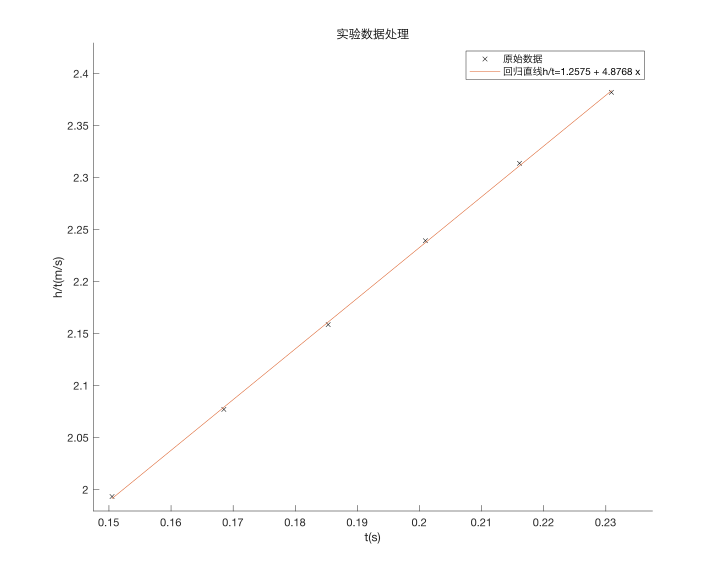
\includegraphics[scale=0.25]{p3.png}
            \caption{$\frac{\Delta h}{\Delta t}-\Delta t$图}\label{图}
        \end{figure}
    \end{minipage}
\end{table}
作图如上右图\ref{图}.
由回归方程$y=1.2575 + 4.8768x$可知,$\frac{1}{2}g=4.8768~\text m/\text s^2$,故$g=9.7536~\text m/\text s^2$.
同理,对小球(表\ref{小球})、圆柱(表\ref{圆柱}),也可求出回归方程$y=1.3491 + 4.5705 x$(图\ref{p4})、$y=1.4367 + 4.2540 x$(图\ref{p5}).
\begin{figure}[H]%插入图片
    \centering%图片居中
    \subfigure[小球]{%小图一的名称
        \includegraphics[scale=0.17]{p4.png}\label{p4}
        }
    \quad
    \subfigure[圆柱]{%小图二的名称
        \includegraphics[scale=0.17]{p5.png} \label{p5} 
        }
    \caption{$\frac{\Delta h}{\Delta t}-\Delta t$图}%总的图名称
\end{figure}
分别求得$g=9.1410~\text m/\text s^2$,$g=8.5080~\text m/\text s^2$,因数据较少,且小球、小圆柱较轻,故误差较大.
\subsubsection{误差分析}
相对于合肥本地的重力加速度$g=9.7947~\text m/\text s^2$,
对于大球的数据,有相对误差$\frac{\Delta g}{g}=0.41961\%$;
对于小球的数据,有相对误差$\frac{\Delta g}{g}=6.6740\%$;
对于圆柱的数据,有相对误差$\frac{\Delta g}{g}=13.137\%$.
显而易见,大球的数据由于测量组数较多,且大球较重使得空气阻力影响小,误差很小.
但是,对于小球和圆柱的数据,由于测量组数很少,且其受空气阻力影响大,测出重力加速度的误差非常之大,是无效的数据.

大球的实验误差主要来自系统误差(即数字毫秒计对时间的测量误差、卷尺对高度测量的误差,还有空气阻力产生的误差)、偶然误差(即读长度时的误差).

\subsection{单摆法测重力加速度}
\subsubsection{数据处理}
对表\ref{单摆}的数据进行处理,得
\begin{table}[H]
    \begin{center}
        \begin{tabular}{ccc}
            \toprule
            $l$/m & $T$/s\\
            \midrule
            0.5200 & 1.46826 \\
            0.5200 & 1.45771 \\
            0.5200 & 1.44600 \\
            0.5200 & 1.44643 \\
            0.5200 & 1.42500 \\
            0.7050 & 1.68386 \\
            \bottomrule
        \end{tabular}
        \caption{处理后数据}
    \end{center}
\end{table}
从而$\overline{T_{1^{st}}}=1.44868~\text s$,$\overline{l_{1^{st}}}=0.5200~$m.
于是$g=\overline{l_{1^{st}}}(\frac{2\pi}{\overline{T}})^2=9.782~\text m/\text s^2$.
对于$l=0.7050~$m的情况,同理可得$g=9.816~\text m/\text s^2$.

\subsubsection{误差分析}
相对于合肥本地的重力加速度$g=9.7947~\text m/\text s^2$,
对于摆长$l=0.5200~$m,有相对误差$\frac{\Delta g}{g}=0.13195\%$;
对于摆长$l=0.7050~$m,有相对误差$\frac{\Delta g}{g}=0.21835\%$.
\\\suo $l=0.5200~$m时,对$l$,有
\begin{equation*}
    \begin{aligned}
        U_{l_{0.95}}&=\sqrt{\left(t_{0.95}u_A\right)^2+\left(\frac{k_{0.95}\Delta _B}{C}\right)^2}
        \approx\frac{1.960\sqrt{\Delta _{\text{仪}}^2+\Delta_{\text{估}}^2}}{3}\\
        &=\frac{49}{75}\sqrt{0.02^2+0.005^2}~\text m\approx0.01247~\text m
    \end{aligned}
\end{equation*}
对T,有
\begin{equation*}
    \begin{aligned}
        U_{T_{0.95}}&=\frac{1}{n}\sqrt{\left(t_{0.95}u_A\right)^2+\left(\frac{k_{0.95}\Delta _B}{C}\right)^2}
        \approx\frac{1}{70}\sqrt{\left(2.78\sqrt{\frac{\sum_{i=1}^5\left(t_i-\overline{t}\right)^2}{5\left(5-1\right)}}\right)^2+\left(\frac{1.960\sqrt{0.01^2}}{3}\right)^2}~\text s\\
        &\approx0.0200374~\text s
    \end{aligned}
\end{equation*}
故总
\begin{equation*}
    \begin{aligned}
        \frac{U_{g_{0.95}}}{g}&=\sqrt{\left(\frac{U_{l_{0.95}}}{l}\right)^2+4\left(\frac{U_{T_{0.95}}}{T}\right)^2}
        \approx\sqrt{\left(\frac{0.01247}{0.5200}\right)^2+4\left(\frac{0.0200374}{1.44868}\right)^2}\approx2.76817\%
    \end{aligned}
\end{equation*}
所以$g=9.782\pm0.2708~\text m/\text s^2$,结果未达到设计要求.
原因是测的周期数过少,设计方案时(附件2)预计要测$100T$左右,但实验时只测了$70T$,导致随机误差、仪器允差不能很好地削弱.

\section{思考}
\subsection{自由落体法测重力加速度}
实际工作中,很难利用$x-t$公式$h=\frac{1}{2}gt^2$精确测量$g$,因为在按下START按钮准备释放时,由于电磁铁仍有剩磁,导致物体不能同时开始下落,
往往会延迟最高达$20~$ms左右,从而很难精确地测得下落时间$t$.因此很难利用$x-t$公式来精确测量$g$.因此我们选用双光电门法,来提高测量时间的准确度.

那么,在布置光电门时,由于物体下落速度开始满而后来快,因此为了提高光电门1对物体通过对时刻的感应精度,应尽可能减小物体在光电门中滞留的时间,
意即光电门1点位置应在条件允许的情况下尽可能偏低.另外,由于实验方案设计为用小球通过两光电门之前路程点平均速度来测量$g$,所以为了减小相对误差,
应使两光电门之间的距离尽可能大,以延长时间,减小测量时间的误差在总时间中的占比,即相对误差,从而获得更准确的数据.

在进行完本实验后,容易看出,利用相同的实验装置,可以设计出其他测量$g$的方法:由$h=\frac{1}{2}gt^2$得$t=\sqrt{\frac{2h}{g}}$.
从而$\left|\Delta t\right|=\sqrt{\frac{2}{g}}\left|\sqrt{h_2}-\sqrt{h_1}\right|$.作$\left|\Delta t\right|-\left|\sqrt{h_2}-\sqrt{h_1}\right|$图,
则斜率$k=\sqrt{\frac{2}{g}}$,从而$g$可求.

\subsection{单摆法测重力加速度}
对于单摆法测重力加速度,误差来源有以下两个方面:
\begin{enumerate}
    \item \emph{系统误差}~~~单摆法测重力加速度的实验装置本身就较为粗糙,如用米尺测量摆长不够精准(虽然理论上在规定的不确定度范围内,但无法进一步获得精确度极高的数据),
    细线的重量、空气阻力不可忽略,小球的质量过轻,秒表计时不够精确等等.
    \item \emph{偶然误差}~~~每个人都有一定的反应时间,不可能在小球通过中心线的同时立刻掐停秒表;在读取长度时也会有偶然误差等等.
\end{enumerate}
改进方法:

增加摆长;减小摆角;如果可能的话,采用完整版的单摆周期公式;选用质量更轻的摆线;增加摆球质量;使用更高精度的尺测量摆长;
在立杆上加装光电门,以摆线遮挡光线为信号,用计算机计时,极大地减小人工计时延迟产生的误差;
将装置置于真空中,减小空气阻力产生的影响;等等等等.

\end{document}